\begin{question}
The aim of this question is to develop a dynamic network to
generate prime numbers.  The network will be based on the sieve of
Eratosthenes, a technique developed by the ancient Greek polymath
Eratosthenes.  The idea is as follows.  To generate all the primes up to~$n$,
we start by writing down all the integers from~$2$ to~$n$.  We then repeatedly
mark the smallest number as a prime, and remove all multiples of it.  We
repeat until all numbers have been dealt with.  Hence on the
first step, we identify $2$ as prime, and remove all even numbers; on the second
step, we identify~$3$ as prime, and remove all multiples of~$3$; and so on.
Below is the result for $n = 20$, with the identified primes ringed.
%
\begin{center}\small
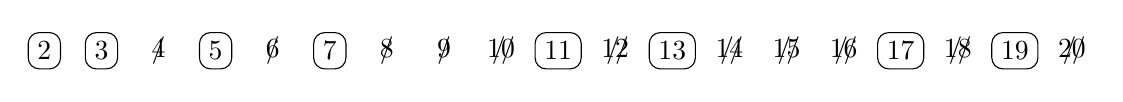
\begin{tikzpicture}[xscale = 0.725] 
\foreach \x in {2,3,5,7,11,13,17,19} 
  \draw (\x,0) node[draw, rounded corners]{$\x$};
\foreach \x in {4,6,8,9} \draw (\x,0) node{$\x\!\!\!/$};
\foreach \x in {10,12,14,15,16,18,20} \draw (\x,0) node{$\x\!\!\!\!\!/\!/$};
%\foreach \x in {2,...,12} \draw(\x,0) node{$\x$};
\end{tikzpicture}
\end{center}

\begin{enumerate}
\item Write a function
\begin{scala}
  private def filter(in: ??[Int], out: !![Int], k: Int) = thread{...}
\end{scala}
which copies values from~|in| to~|out|, but removes all multiples of~|k|.

\item Use |filter| and recursion to write a function
\begin{scala}
  private def sieve(in: ??[Int], out: !![Int]): ThreadGroup = thread{...}
\end{scala}
which copies values from~|in| to~|out|, but removes all multiples of any value
that has been previously input.  

\item Hence write a function
\begin{scala}
  private def primes(out: !![Int], n: Int): ThreadGroup =
\end{scala}
that generates the primes up to~|n|, and sends them on~|out|.  You might need
to adapt your earlier definitions to achieve termination. 
\end{enumerate}
\end{question}

%%%%%%%%%%%%%%%%%%%%%%%%%%%%%%%%%%%%%%%%%%%%%%%%%%%%%%%

\begin{answerI}
My code is below.  The |generator| component generates the numbers from |2|
to~|n|.  The channel is closed to show the end of the stream; and other
components pass this signal on.  The definition of |sieve| generates a new
thread executing |filter| for each input that is not a multiple of an earlier
one.
%
\begin{scala}
  /** Component that passes values from £in£ to £out£, removing multiples of £n£. */
  private def filter(in: ??[Int], out: !![Int], k: Int) = thread{
    repeat{ val m = in?(); if(m%k != 0) out!m }
    out.endOfStream()
  }

  /** Component that sieves values received on £in£, removing multiples of
    * earlier values, but passing remainder on £out£. */
  private def sieve(in: ??[Int], out: !![Int]): ThreadGroup = thread{
    attempt{
      val k = in?(); out!k; val mid = new SyncChan[Int]
      run(filter(in, mid, k) || sieve(mid, out))
    }{ out.endOfStream() }
  }

  /** Component that sends values £2 to n£ on £c£. */
  private def generator(c: !![Int], n: Int) = thread{
    for(i <- 2 to n) c!i
    c.endOfStream()
  }

  /** Network to generate the primes up to £n£, and send them on £out£. */
  private def primes(out: !![Int], n: Int): ThreadGroup = {
    val in = new SyncChan[Int]
    generator(in, n) || sieve(in, out) 
  }
\end{scala}
\end{answerI}
